\documentclass[11pt, addpoints, answers]{exam}

\usepackage{amsmath, amssymb, euler}
\usepackage{xcolor}
\usepackage{tikz, tikz-qtree, drawstack}
\usepackage{physics}
\usepackage{algorithm, algorithmicx, algpseudocode}
\usepackage[shortlabels]{enumitem}

\newcommand{\red}[1]{\textcolor{red}{#1}}

% For inserting code snippets.
\usepackage{listings}
\lstset{
    columns = fixed,
    basewidth = {0.5em},
    breaklines = true,
    backgroundcolor = \color{white},
    keywordstyle = \color[RGB]{40, 40, 255},
    numberstyle = \footnotesize\color{darkgray},
    commentstyle = \ttfamily\color{violet},
    basicstyle = \ttfamily,
    stringstyle = \ttfamily\color[RGB]{128, 0, 0},
    showstringspaces = false,
    language = {[11]C++},
    escapechar = \@
}
\lstnewenvironment{cpp}[1][]{\lstset{language = {[11]C++}, #1}}{}

\usepackage{tikz}
\usepackage{algorithmicx}

% headers, footers, titles
\newcommand{\CourseName}{CS101 Algorithms and Data Structures}
\newcommand{\HomeworkNO}{Homework 9}
\newcommand{\DueDate}{Due date: December 18, 2023, at 23:59}

\pagestyle{headandfoot}
\runningheadrule
\runningheader{\CourseName}{\HomeworkNO}{\DueDate}
\runningfooter{}{\thepage}{}

\title{
    \CourseName\\
    Fall 2023\\
    \HomeworkNO
}
\author{}
\date{\DueDate}

% formats of questions, choices, points, etc.
\qformat{\textbf\thequestion. (\totalpoints\ points) \thequestiontitle\hfill}
\pointname{'}
\CorrectChoiceEmphasis{\color{blue}}
\SolutionEmphasis{\color{blue}}

% We frequently use this font.
\newcommand{\ttt}{\texttt}
\newcommand{\bluett}[1]{\textcolor{blue}{\ttt{#1}}}

\begin{document}

\maketitle

\begin{enumerate}
    \item Please write your solutions in English.
    \item Submit your solutions to gradescope.com.
    \item Set your FULL name to your Chinese name and your STUDENT ID correctly in Account Settings.
    \item If you want to submit a handwritten version, scan it clearly. \ttt{CamScanner} is recommended.
    \item When submitting, match your solutions to the problems correctly.
    \item No late submission will be accepted.
    \item Violations to any of the above may result in zero points.
\end{enumerate}

\begin{questions}

    \newpage

    \titledquestion{Multiple Choices}

Each question has \textbf{one or more} correct answer(s). Select all the correct answer(s). For each question, you will get 0 points if you select one or more wrong answers, but you will get 1 point if you select a non-empty subset of the correct answers.

Write your answers in the following table.

%%%%%%%%%%%%%%%%%%%%%%%%%%%%%%%%%%%%%%%%%%%%%%%%%%%%%%%%%%%%%%%%%%%%%%%%%%%
% Note: The `LaTeX' way to answer a multiple-choices question is to replace `\choice'
% with `\CorrectChoice', as what you did in the first question. However, there are still
% many students who would like to handwrite their homework. To make TA's work easier,
% you have to fill your selected choices in the table below, no matter whether you use 
% LaTeX or not.
%%%%%%%%%%%%%%%%%%%%%%%%%%%%%%%%%%%%%%%%%%%%%%%%%%%%%%%%%%%%%%%%%%%%%%%%%%%

\begin{table}[htbp]
    \centering
    \begin{tabular}{|p{2cm}|p{2cm}|p{2cm}|p{2cm}|}
        \hline
        (a) & (b) & (c) & (d) \\
        \hline
        %%%%%%%%%%%%%%%%%%%%%%%%%%%%%%%%%%%%%%%%%%%%%%%%%%%%%%%%%%
        % YOUR ANSWER HERE.
        AD  & BCD & AB  & D    \\
        %%%%%%%%%%%%%%%%%%%%%%%%%%%%%%%%%%%%%%%%%%%%%%%%%%%%%%%%%%
        \hline
    \end{tabular}
\end{table}

\begin{parts}
    \part[2] Which of the following operations on a \textbf{Linked List} take constant time?

    \begin{choices}
        \CorrectChoice Given a pointer $h$ which points  to the head node of a linked list, we want to erase the head node.
        \choice Given a pointer $h$ which points to the head node of a linked list, we want to gain access to the last element of the linked list.
        \choice Given a pointer $p$ which points to a node in a linked list, we want to gain access the previous node of $p$.
        \CorrectChoice Given a pointer $p$ which points to a node in a linked list, we want to insert an element after $p$.
    \end{choices}

    \part[2] Which of the following statements about arrays and linked-lists are true?

    \begin{choices}
        \choice Inserting an element into the middle of an array takes constant time.
        \CorrectChoice A doubly linked list consumes more memory than a (singly) linked list of the same length.
        \CorrectChoice Given a pointer to some node in a doubly linked list, we are able to gain access to every node of it.
        \CorrectChoice Given a pointer to any node in a linked list, we are able to gain access to the last node.
    \end{choices}

    \part[2] Please evaluate the following reverse-Polish expressions. Which of them are legal reverse-Polish expressions and gives a result greater than 0?

    \begin{choices}
        \CorrectChoice \ttt{2 3 2 * + 1 /}
        \CorrectChoice \ttt{1 2 4 - - 3 *}
        \choice \ttt{1 * 2 - 1 + 5}
        \choice \ttt{2 4 3 1 + * -}
    \end{choices}

    \part[2] Assume we implement a queue with a circular array indexed from $0$ to $n-1$. Now the \ttt{front} pointer is at index $a$, and the \ttt{back} pointer is at index $b$. Which of the following best describes the number of the elements in the queue?

    \begin{choices}
        \choice $b-a+1$
        \choice $|b-a+1|$
        \choice $b-a+1+n$
        \CorrectChoice $(b-a+1+n) \mod n$
    \end{choices}


\end{parts}

    \newpage

    \titledquestion{Topological Sort}

Given the following DAG, run topological sort with a queue. Write down the vertex you select and update the in-degree \texttt{ind[i]} of all vertices in each iteration.

\textit{Note: When pushing several vertices into the queue at the same time, push them alphabetically. You are NOT required to show your queue at each step.}

\vspace{1cm}

\begin{figure}[htbp]
    \centering
    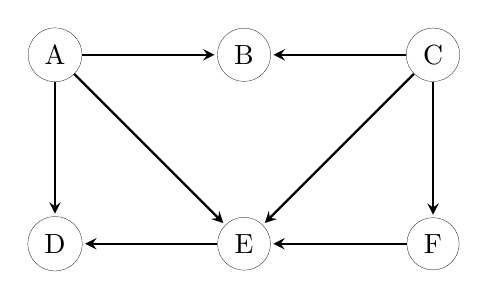
\begin{tikzpicture}[
            > = stealth, % arrow head style
            shorten > = 1pt, % don't touch arrow head to node
            node distance = 1cm, % distance between nodes
            thick, % line style
            scale = 0.8,
        ]
        % Draw the nodes
        \foreach \pos/\i in {
                (-3,3)/A,
                (0,3)/B,
                (3,3)/C,
                (-3,0)/D,
                (0,0)/E,
                (3,0)/F} {
                \node[circle, draw, line width=0.1pt] (\i) at \pos {\i};
            }

        % Draw the edges
        \foreach \b/\e in {
                A/B,
                A/D,
                A/E,
                C/B,
                C/E,
                C/F,
                F/E,
                E/D} {
                \draw[->] (\b) to (\e);
            }
    \end{tikzpicture}\label{fig:Topological_Sort}
\end{figure}
\vspace{0.5cm}

\begin{table}[htbp]
    \begin{center}
        \begin{tabular}{|l|c|l|l|l|l|l|l|}
            \hline
                        & vertex & \texttt{ind[A]}     & \texttt{ind[B]}     & \texttt{ind[C]}     & \texttt{ind[D]}     & \texttt{ind[E]}     & \texttt{ind[F]}     \\ \hline
            initial     & /      & \textcolor{blue}{0} & \textcolor{blue}{2} & \textcolor{blue}{0} & \textcolor{blue}{2} & \textcolor{blue}{3} & \textcolor{blue}{1} \\ \hline
            iteration 1 & A      & \textcolor{blue}{0} & \textcolor{blue}{1} & \textcolor{blue}{0} & \textcolor{blue}{1} & \textcolor{blue}{2} & \textcolor{blue}{1} \\ \hline
            iteration 2 & C      & \textcolor{blue}{0} & \textcolor{blue}{0} & \textcolor{blue}{0} & \textcolor{blue}{1} & \textcolor{blue}{1} & \textcolor{blue}{0} \\ \hline
            iteration 3 & B      & \textcolor{blue}{0} & \textcolor{blue}{0} & \textcolor{blue}{0} & \textcolor{blue}{1} & \textcolor{blue}{1} & \textcolor{blue}{0} \\ \hline
            iteration 4 & F      & \textcolor{blue}{0} & \textcolor{blue}{0} & \textcolor{blue}{0} & \textcolor{blue}{1} & \textcolor{blue}{0} & \textcolor{blue}{0} \\ \hline
            iteration 5 & E      & \textcolor{blue}{0} & \textcolor{blue}{0} & \textcolor{blue}{0} & \textcolor{blue}{0} & \textcolor{blue}{0} & \textcolor{blue}{0} \\ \hline
            iteration 6 & D      & \textcolor{blue}{0} & \textcolor{blue}{0} & \textcolor{blue}{0} & \textcolor{blue}{0} & \textcolor{blue}{0} & \textcolor{blue}{0} \\ \hline
        \end{tabular}
    \end{center}\label{tab:Topological_Sort_Answer}
\end{table}
\vspace{0.5cm}



\begin{parts}
    \part[3] Fill in the table above.
    \part[2] What is the topological order that you obtain?
    \part[3] How many different topological orders starting with A does this graph have?
    Write them down.
\end{parts}

\begin{solution}
    \begin{enumerate}
        \item ACBFED
        \item 4. ACBFED, ACFBED, ACFEBD, ACFEDB
    \end{enumerate}
\end{solution}

    \newpage

    \titledquestion{Array Section}

Given an upper bound \(M\) and a sequence of positive integers \(A=\langle a_1,\cdots,a_n\rangle\) where \(\forall i \in [1, n], a_i \leq M\), we want to divide it into several consecutive sections so that the sum of each section is less than or equal to the upper bound \(M\), and the number of sections is minimized.

For example, if \(M=6\) and \(A=\langle 4,2,4,5,1\rangle\), the minimum number of sections is \(3\), and there are two ways to divide the sequence \(A\) into \(3\) sections: \(\langle 4\rangle,\langle 2,4\rangle,\langle 5,1\rangle\) and \(\langle 4,2\rangle,\langle 4\rangle,\langle 5,1\rangle\).

Design a greedy algorithm to find the minimum number of sections in \(\Theta(n)\) time, and prove its correctness.

\begin{parts}
    \part[2] Describe your algorithm in \textbf{pseudocode}.
    \part[2] Analyse the time complexity based on your \textbf{pseudocode}.
    \part[1] How to define the sub-problem $g(i)$ in your algorithm?
    \part[2] How do you solve $g(i)$ by calling $g(i-1)$ recursively?
    \part[2] Prove the correctness of solving $g(i)$ by calling $g(i-1)$.
\end{parts}

\begin{solution}
    \begin{enumerate}
        \item \textbf{Pseudocode:}\\
              Define two iterators it which starts at the first element of the array.
              Answer is the number of sections we need. Length is the length of array A.
              Current is the sum of elements in the array which is less than or equal to M.
              \begin{algorithm}[H]
                  \color{blue}
                  \begin{algorithmic}[1]
                      \Function {find$\_$minimum$\_$sections}{array A, M}
                      \State it $\gets$ 0
                      \State answer $\gets$ 0
                      \State length $\gets$ A.size()
                      \State current $\gets$ 0
                      \While {it != length}
                      \If {current + A[it] $<$ M}
                      \State current += A[it]
                      \State it++
                      \ElsIf {current + A[it] = M}
                      \State current $\gets$ 0
                      \State answer += 1
                      \State it++
                      \Else
                      \State current $\gets$ A[it]
                      \State answer += 1
                      \State it++
                      \EndIf
                      \EndWhile
                      \EndFunction
                  \end{algorithmic}
              \end{algorithm}
    \end{enumerate}
\end{solution}
\newpage
\begin{solution}
    \begin{enumerate}
        \item \textbf{Analysis:}
              Outside the loop the time complexity is $\theta(n)$. \\
              Inside the loop the whole time complexity is $\frac{5}{12} \theta(2) + \frac{1}{6} \theta(3) + \frac{5}{12} \theta(3)$,
              which is $\theta(1)$. \\
              Thus the whole time complexity is $\theta(n) + n \cdot \theta(1) = \theta(n)$.
        \item The sub-problem g(i) is the minimun number of section in A from the first element to the ith element.
        \item If after adding A[i] to the current in the pseudocode, current is larger than or equal to M, then g(i) = g(i-1)+1; otherwise, g(i) = g(i-1).
        \item Knowing that g(i-1) is the best way of dividing, and we assume that there exist a better solution for g(i), called h(i).
              Then there must be a inequation that the number of sections in h(i) is less than or equal to those in g(i).
              We know that g(i) equals to g(i-1) or g(i-1)+1, thus h(i) is sometimes g(i-1) when g(i) is g(i-1)+1.
              When g(i) equals to g(i-1)+1, it means the ith element can not be put into the last section, while in h(i) the ith can.
              Since the order will not change, there must be some elements in the last section of g(i) not belonging to the last section in h(i).
              For these elements, they can be regarded as new elements which should be added into g(i-2).
              Repeat the operations above until g(1)(h(1) should add new elements to g(1)), then we can know that h(1) is obviously larger than or equal to g(1), contradicting to the condition that h(i) is less than or equal to those in g(i).
              Thus solving g(i) by calling g(i-1) is correct.
    \end{enumerate}
\end{solution}

    \newpage

    \titledquestion{Minimum Cost Refueling}

You are planning to from city A to city B on a highway.
The distance between A and B is $d$ kilometers.
The vehicle departs with $f_0$ units of fuel.
Each unit of fuel makes the vehicle travel one kilometer.

There are $n$ gas stations along the way.
The $i$-th station is situated $p_i$ kilometers away from city A.
Note that $0<p_1<p_2<\cdots<p_n<d$.

If the vehicle chooses to refuel at the $i$-th station, $f_i>0$ units would be added to the fuel tank whose capacity is unlimited, which costs you \$$c_i$.
    You have a budget $B$, which means that the sum of costs on refueling is at most \$$B$.

    Please design a \textbf{dynamic programming} algorithm that returns \textbf{the minimum cost of refueling} to make sure the vehicle reaches the destination if the vehicle can reach the target, or returns $\varnothing$ if your budget is not enough or the fuel is not enough to support you to reach city B.

\begin{parts}
    \part[3] Define the subproblems for $i\in[0,n],j\in[0,B]$: $OPT(i, j)=$ the maximum distance you can drive if you spend \textbf{at most} \$$j$ among the first $i$ stations. Give your Bellman equation to solve the subproblems.

        \begin{solution}
            \[
                OPT(i,j) =
                \begin{cases}
                    f_0                                     & \case{i=0}                     \\
                    OPT(i-1,j)                              & \case{OPT(i-1,j)<p_i || j<c_i} \\
                    \max \{OPT(i-1,j), OPT(i-1,j-c_i)+f_i\} & otherwise
                \end{cases}
            \]
        \end{solution}

        \part[2] What is the answer to this question in terms of $OPT$?

        \begin{solution}
            Find all O(i,j) which is larger than d.
            Find the minimum j among them. If j is less than or equal to B, return j.
            Otherwise, return $\varnothing$.
        \end{solution}

        \part[1] What is the runtime complexity of your algorithm? (answer in $\Theta(\cdot)$)

    \begin{solution}
        $\Theta(nB)$.
    \end{solution}

\end{parts}

    \newpage

    \ % The empty page

    \newpage

\end{questions}

\end{document}